\chapter{Riconoscitori a stati finiti}
...
\section{Dai riconoscitori ai generatori}
\begin{figure}[H]
    \caption{Automa}
    \centering
    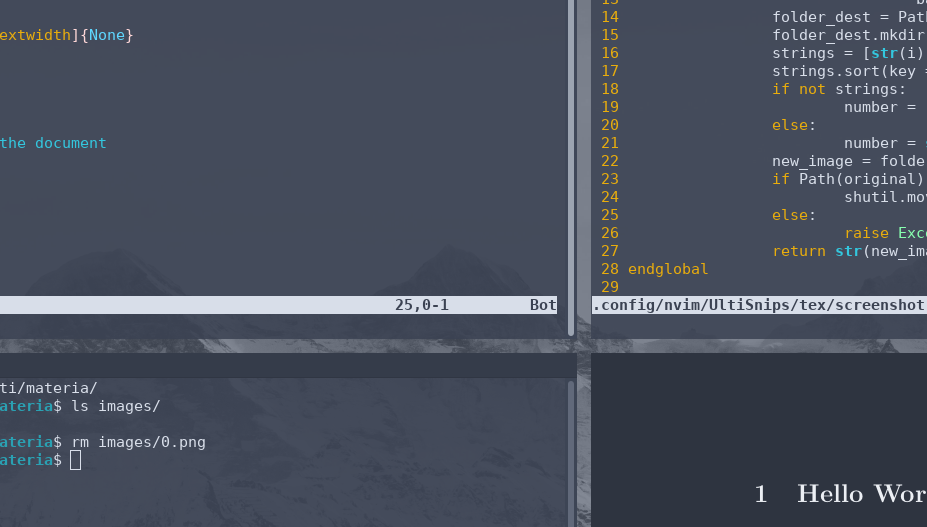
\includegraphics[width=0.8\textwidth]{/home/riccardoob/appunti/linguaggi/images/0.png}
\end{figure}
\setlist{nosep}
Descrivendo a parole le transizioni utili dell'automa:
\begin{itemize}
    \item nello stato I l'automa può accettare:
    \begin{itemize}
        \item il simbolo a e portarsi nello stato A
    \end{itemize}
    \item nello stato A l'automa può accettare:
    \begin{itemize}
        \item il simbolo b e poi fermarsi
        \item il simbolo a e riportarsi nello stato A stesso
    \end{itemize}
    \item nello stato finale F l'automa puà accettare:
    \begin{itemize}
        \item nessun simbolo
    \end{itemize}
\end{itemize}
\setlist{}

Se si sostituisce la parola accettare alla parola generare, si nota che l'automa può essere considerato come generatore.

Si può definire un \textbf{mapping} tra:
\begin{itemize}
    \item stati $\longleftrightarrow$ simboli non terminali
    \item transizioni $\longleftrightarrow$ produzioni
    \item scopo $\longleftrightarrow$ uno stato particolare
\end{itemize}

É possibile automatizzare la costruzione di un RSF a partire dalla grammatica o viceversa.

\begin{multicols}{2}
Grammatica regolare a \underline{destra}:
\begin{itemize}
    \item scopo = stato iniziale: $I$
    \item stato finale: $F$
    \begin{itemize}
        \item $S \rightarrow a\ A$
        \item $A \rightarrow a\ A\ |\ b$
    \end{itemize}
\end{itemize}
Grammatica regolare a \underline{sinistra}:
\begin{itemize}
    \item scopo = stato finale: $F$
    \item stato inziale: $I$
    \begin{itemize}
        \item $S \rightarrow A\ b$
        \item $A \rightarrow A\ a\ |\ a$
    \end{itemize}
\end{itemize}
\end{multicols}

Lo stato finale F non si considera perché non ha archi uscenti.

Come arrivare a queste grammatiche?

\subsection{Mapping RSF $\longleftrightarrow$ grammatica}

Si immagini un osservatore che, stando in ogni stato, guardi da ogni stato:

\begin{multicols}{2}
    \begin{itemize}
        \item \underline{dove si va}
        \begin{itemize}
            \item la freccia col \textbf{simbolo terminale}
            \item lo stato \textbf{successivo}
        \end{itemize}
        \item \underline{da dove viene}
        \begin{itemize}
            \item lo stato \textbf{precendente}
            \item la freccia col \textbf{simbolo terminale}
        \end{itemize}
    \end{itemize}
\end{multicols}

\subsubsection{Mapping tra automa riconoscitore e grammatica}
Tra la grammatica e il riconoscitori si riconoscono le seguenti corrispondenze:
\begin{itemize}
    \item \textbf{stati} dell'automa $\longleftrightarrow$ \textbf{metasimboli} della grammatica
    \item \textbf{transizioni} dell'automa $\longleftrightarrow$ \textbf{produzioni} della grammatica
    \item \textbf{uno stato} dell'automa $\longleftrightarrow$ \textbf{scopo} della grammatica
\end{itemize}
Se la grammatica è \underline{regolare a destra} si ottiene un automa \underline{top-down}.\\
Se la grammatica è \underline{regolare a sinistra} si ottiene un automa \underline{bottom-up}.\\
In modo analogo si ottengono grammatiche destra/sinistra interpretando un RSF in modo top-down/bottom-up

\noindent
Ad esempio:

In questo caso gli stati iniziale e finale sono anche \underline{stati di transito}.
\begin{figure}[H]
    \begin{subfigure}{0.5\textwidth}
        \caption{Traduzione grammatica}
        \centering
        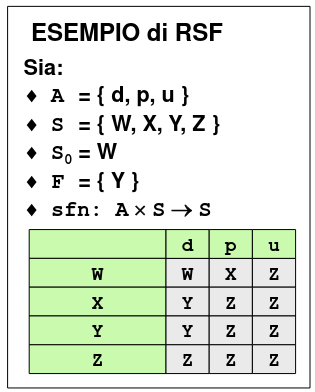
\includegraphics[width=0.4\linewidth]{/home/riccardoob/appunti/linguaggi/images/1.png}
    \end{subfigure}% 
    \begin{subfigure}{0.5\textwidth}
        \caption{Riconoscitore}
        \centering
        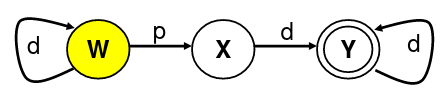
\includegraphics[width=0.4\linewidth]{/home/riccardoob/appunti/linguaggi/images/2.png}
    \end{subfigure}
\end{figure}

Per passare dall'automa alla grammatica si analizzano i collagamenti degli stati e si ricavano le trasformazioni:
\\
\begin{multicols}{2}
    \noindent
    \begin{equation*}
        \begin{aligned}[t]
        &W \rightarrow d\ W &&|\ p\ X\\
        &X \rightarrow d\ &&|\ d\ Y\\
        &Y \rightarrow d\ &&|\ d\ Y
        \end{aligned}
    \end{equation*}
    \begin{equation*}
        \begin{aligned}[t]
        &Y \rightarrow X\ d &&|\ Y\ d\\
        &X \rightarrow p\ &&|\ W\ p\\
        &W \rightarrow d\ &&|\ W\ d
        \end{aligned}
    \end{equation*}    
\end{multicols}

\subsection{Riconoscitori top down}
\textbf{Derivazione top-down}\\
Si parte dallo scopo della grammatica e si tenta di coprire la frase data tramite produzioni successive.\\
\begin{multicols}{2}
Data una grammatica regolare lineare a \underline{destra}, il riconoscitore:

\begin{itemize}
    \item ha tanti \textbf{stati} quanti i \underline{simboli non terminali}
    \item ha come \textbf{stato iniziale} lo \underline{scopo S}
    \item per ogni regola del tipo $X \rightarrow x\ Y$, l'automa con ingresso $x$ passa dallo stato $X$ allo stato $Y$
    \item per ogni regola del tipo $X \rightarrow x$, l'automa con ingresso $x$ passa dallo stato $X$ allo stato finale $F$
\end{itemize}
\columnbreak
\textbf{Esempio}\\
Sia G una grammatica lineare a destra caratterizzata dalle seguenti produzioni:
\begin{itemize}
    \item $S \rightarrow a\ B\ |\ b$
    \item $B \rightarrow b\ S\ |\ a$
\end{itemize}
\begin{multicolfigure}
    \centering
    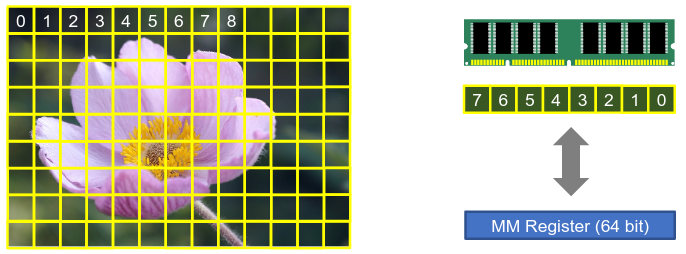
\includegraphics[width=0.4\textwidth]{/home/riccardoob/appunti/linguaggi/images/3.png}
\end{multicolfigure}
\end{multicols}

\subsection{Riconoscitori bottom up}
\begin{multicols}{2}
Data una grammatica regolare lineare a \underline{sinistra}, il riconoscitore:
\begin{itemize}
    \item ha tanti \textbf{stati} quanti i \underline{simboli non terminali}
    \item ha come \textbf{stato finale} lo \underline{scopo S}
    \item per ogni regola del tipo $X \rightarrow Y\ x$, l'automa con ingresso $x$ passa dallo stato $Y$ allo stato $X$
    \item per ogni regola del tipo $X \rightarrow x$, l'automa con ingresso $x$ passa dallo stato iniziale $I$ allo stato $X$
\end{itemize}
\columnbreak
\textbf{Esempio}\\
Sia G una grammatica lineare a sinistra caratterizzata dalle seguenti produzioni:
\begin{itemize}
    \item $S \rightarrow B\ a\ |\ b$
    \item $B \rightarrow S\ b\ |\ a$
\end{itemize}
\begin{multicolfigure}
    \centering
    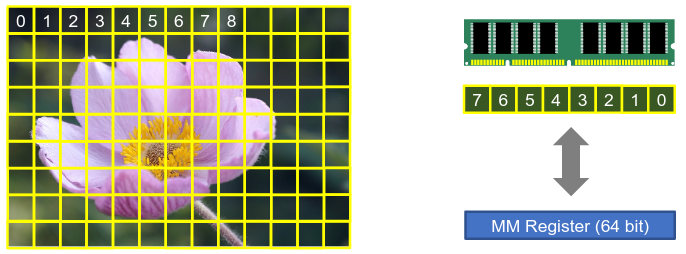
\includegraphics[width=0.4\textwidth]{/home/riccardoob/appunti/linguaggi/images/3.png}
\end{multicolfigure}
\end{multicols}

\subsection{Dall'automa alle grammatiche}
Dato un automa riconoscitore, se ne possono trarre sia una grammatica regolare a \underline{destra} (interpretazione top-down) che una grammatica regolare a \underline{sinistra} (interpretazione bottom-up).
\noindent\\
\begin{multicols}{2} 
Caso generico
\begin{itemize}
    \item top-down:     $A \rightarrow a\ B$
    \item bottom-up:     $A\ a \leftarrow B$
\end{itemize}    
\columnbreak
\begin{multicolfigure}
    \centering
    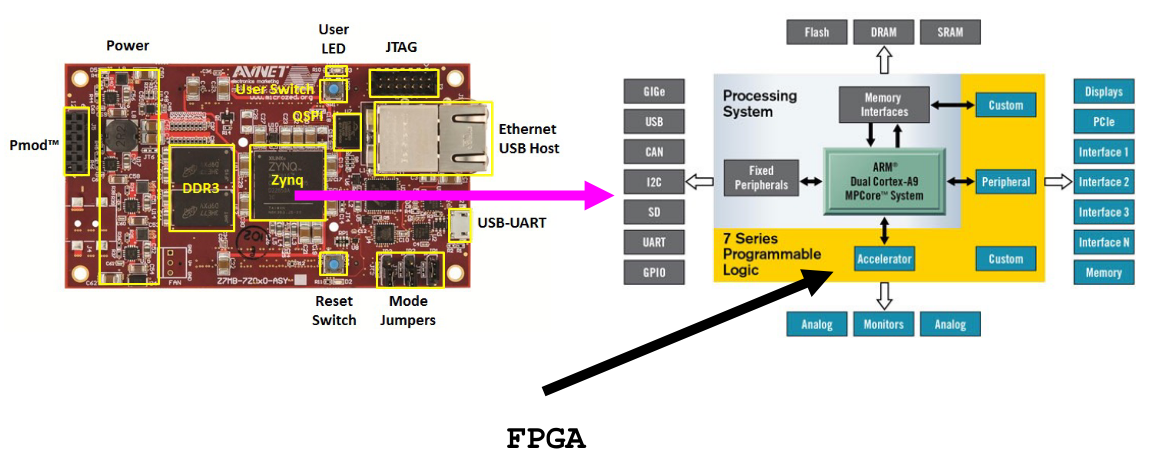
\includegraphics[width=0.5\textwidth]{/home/riccardoob/appunti/linguaggi/images/6.png}
\end{multicolfigure}
\end{multicols}
\begin{multicols}{2}
    \noindent
    Caso iniziale
    \begin{itemize}
        \item top-down:     $S \rightarrow a\ B$
        \item bottom-up:    $I\ a \leftarrow B$
    \end{itemize}
    \begin{multicolfigure}
        \centering
        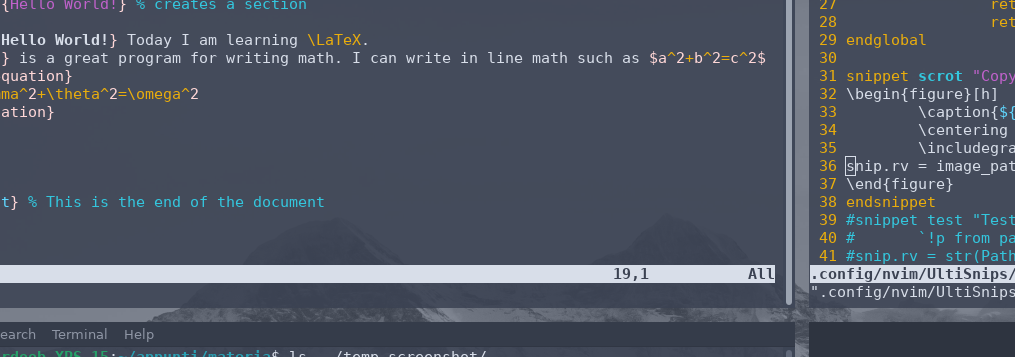
\includegraphics[width=0.5\textwidth]{/home/riccardoob/appunti/linguaggi/images/4.png}
    \end{multicolfigure}
    \columnbreak
    \noindent
    Caso finale
    \begin{itemize}
        \item top-down:     $A \rightarrow a\ F$
        \item bottom-up:    $A\ a \leftarrow S$
    \end{itemize}
    \begin{multicolfigure}
        \centering
        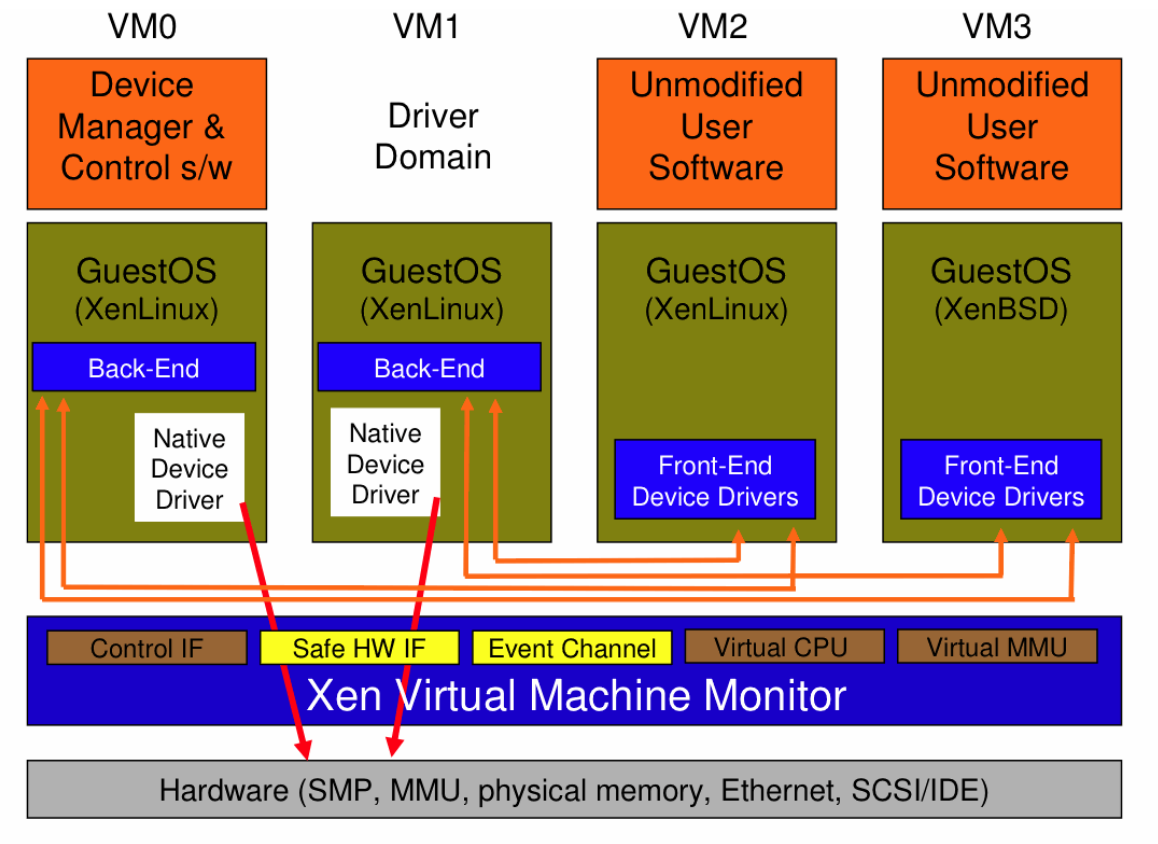
\includegraphics[width=0.5\textwidth]{/home/riccardoob/appunti/linguaggi/images/5.png}
    \end{multicolfigure}
\end{multicols}

\subsubsection{Esempio}

\begin{figure}[H]
    \centering
    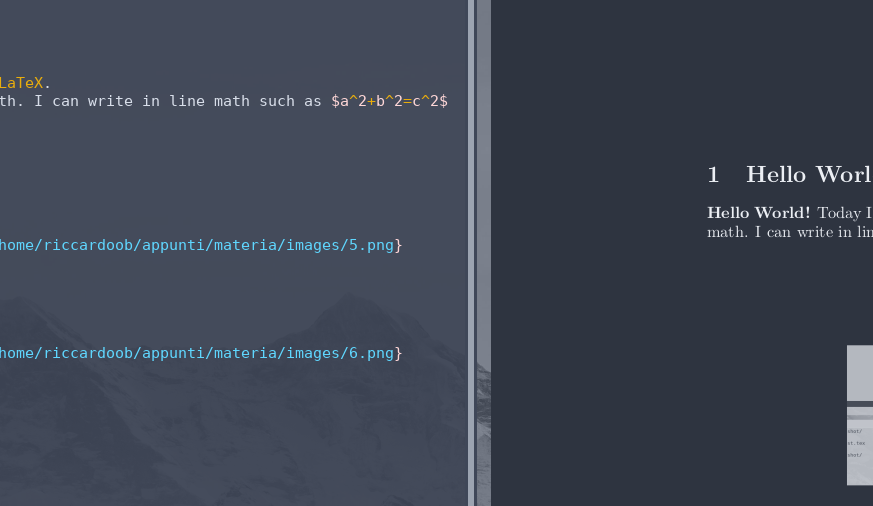
\includegraphics[width=0.4\textwidth]{/home/riccardoob/appunti/linguaggi/images/7.png}
\end{figure}

\setlist{nosep}
\begin{multicols}{2}
\noindent
Analisi top-down (C finale omesso):
\begin{itemize}
    \item $I \rightarrow b\ B$
    \item $I \rightarrow a\ A$
    \item $B \rightarrow a\ A$
    \item $A \rightarrow a\ A$
    \item $B \rightarrow c$
    \item $A \rightarrow c$
\end{itemize}

\columnbreak
\noindent
Analisi bottom-up (C iniziale):
\begin{itemize}
    \item $b \leftarrow  B$
    \item $a \leftarrow  A$
    \item $B\ a \leftarrow  A$
    \item $A\ a \leftarrow  A$
    \item $B\ c \leftarrow  S$
    \item $A\ c \leftarrow  S$
\end{itemize}
\end{multicols}
\setlist{}

\begin{multicols}{2}
\noindent
Grammatica G1 regolare a destra:
\begin{itemize}
    \item $I \rightarrow b\ B\ |\ a\ A$
    \item $B \rightarrow a\ A\ |\ c$
    \item $A \rightarrow a\ A\ |\ c$
\end{itemize}
\begin{multicolfigure}
    \centering
    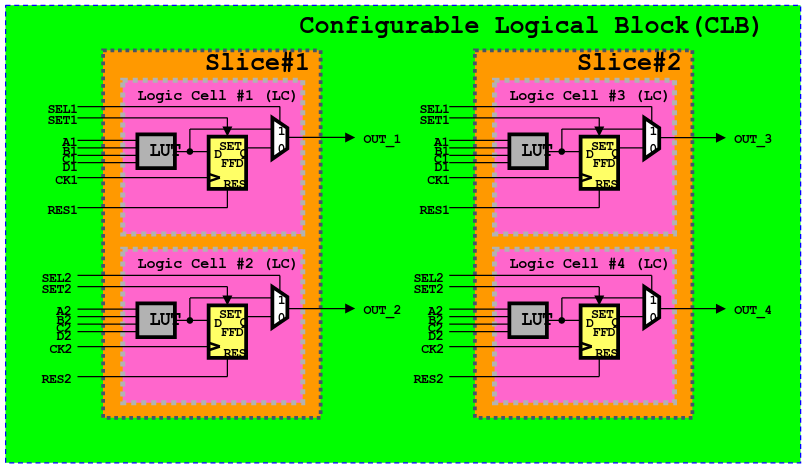
\includegraphics[width=0.7\textwidth]{/home/riccardoob/appunti/linguaggi/images/8.png}
\end{multicolfigure}
\columnbreak
\noindent
Grammatica G2 regolare a sinistra:
\begin{itemize}
    \item $S \rightarrow B\ c\ |\ A\ c$
    \item $A \rightarrow B\ a\ |\ A\ a\ |\  a$
    \item $B \rightarrow b$
\end{itemize}
\begin{multicolfigure}
    \centering
    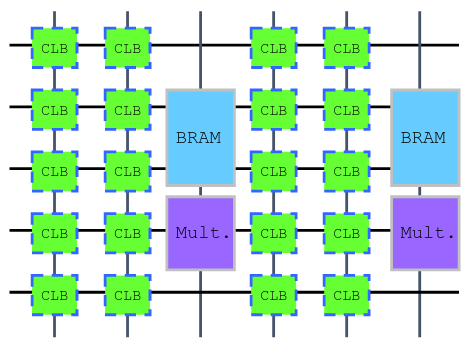
\includegraphics[width=0.7\textwidth]{/home/riccardoob/appunti/linguaggi/images/9.png}
\end{multicolfigure}    
\end{multicols}

\textbf{Esempio multipli stati finali}\\
\begin{figure}[H]
    \centering
    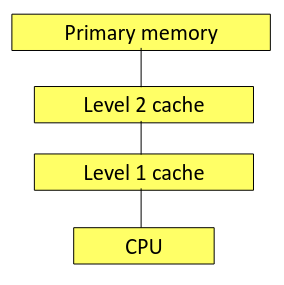
\includegraphics[width=0.4\textwidth]{/home/riccardoob/appunti/linguaggi/images/10.png}
\end{figure}
\newpage
\setlist{nosep}
\begin{multicols}{2}
\noindent
Analisi top-down (regola in più sulla $I$):
\begin{itemize}
    \item $I \rightarrow b\ B\ |\ b$
    \item $I \rightarrow a\ A$
    \item $B \rightarrow a\ A$
    \item $A \rightarrow a\ A$
    \item $B \rightarrow c$
    \item $A \rightarrow c$
\end{itemize}

\columnbreak
\noindent
Analisi bottom-up (C iniziale):
\begin{itemize}
    \item $b \leftarrow  B$
    \item $a \leftarrow  A$
    \item $B\ a \leftarrow  A$
    \item $A\ a \leftarrow  A$
    \item $B\ c \leftarrow  C$
    \item $A\ c \leftarrow  C$
\end{itemize}
\end{multicols}
\setlist{}
L'analisi bottom-up deve scegliere quale scopo adottare, se $B$ o $C$. Per risolvere questo problema si creano due grammatiche in cui si assumono a turno $C \equiv S$ e $B \equiv S$.


\begin{figure}[H]
    \begin{subfigure}{0.5\textwidth}
        \centering
        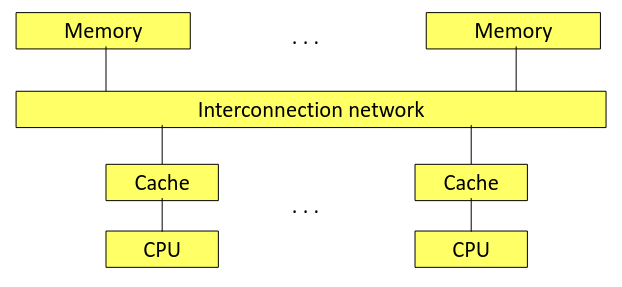
\includegraphics[width=0.7\linewidth]{/home/riccardoob/appunti/linguaggi/images/11.png}
    \end{subfigure}%
    \begin{subfigure}{0.5\textwidth}
        \centering
        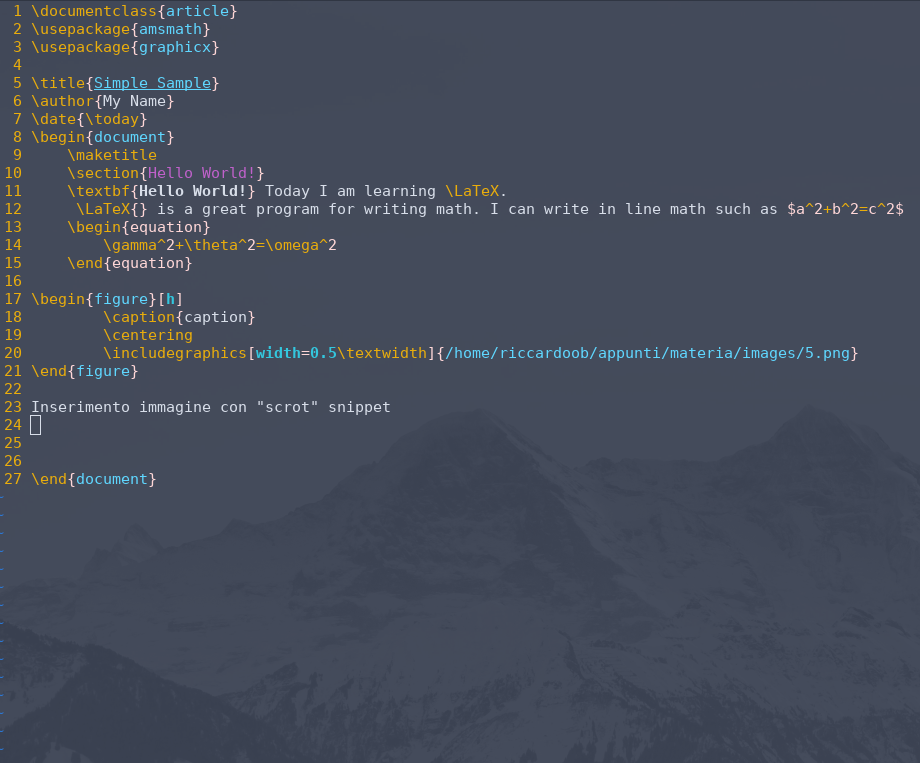
\includegraphics[width=0.7\linewidth]{/home/riccardoob/appunti/linguaggi/images/12.png}
    \end{subfigure}

\end{figure}

\subsubsection{Caso generale}
Nel caso bottom-up, in presenza di più stati finali:
\begin{itemize}
    \item si assume come (sotto)scopo $S_k$ uno stato finale per volta
    \item si scrivono le regole bottom-up corrispondenti
    \item si esprime il linguaggio complessivo come unione dei vari sotto-linguaggi, definendo lo \underline{scopo globale} come $S \rightarrow S_1\ |\ S_2\ |\ \cdots\ |\ S_n$
\end{itemize}


